%%%%%%%%%%%%%%% Testing %%%%%%%%%%%%%%%%%%%%%%%%%
\section{Testing}
\label{sec:testing}

In this section we will explain shortly the testing processes we carried on for
this project. As it was explained in Section \ref{section:methodology-spiral}, we have followed a spiral model,
therefore we have performed testing tasks for each iteration (see Table
\ref{table:iterations}).

\subsection{Functionalities verification}

In order to verify the code, we have performed several tests which assure it
works accordingly to its expected behavior. This was performed in a low
level (after finishing every functionality) and in a high level (after every
iteration or before every demonstration). We also stressed on being sure the
application responds correctly in extreme cases like:
\begin{itemize}
  \item Lack of local/remote applications.
  \item No membership in any community.
  \item The network is down.
  \item \ldots
\end{itemize}

There was also a special interest in assuring all the functionalities related
to the visibility of the applications, tags, etc. work properly due to its
straight relationship with privacy protection.

As we will see in Section \ref{subsubsec:testing-users-study}, a preliminary
version (iterations 1 and 2) was successfully tested in an
users evaluation in December 2008, and another users evaluation is scheduled
in October 2009. The current version of the project have passed successfully
all the tests we performed and we can assure it offers all the expected
functionalities described in the previous sections, so it is ready for being
tested in this new users evaluation. The feedback obtained after carrying on
that process will be very valuable to improve it in the future.

\subsection{OS compatibility}

This project has been totally developed under GNU/Linux, concretely under
Ubuntu 8.04 and 8.10.
All the bundles created for this project have been tested successfully under
different versions of GNU/Linux and Windows XP (see Figure
\ref{img:testing-win-linux}) for both subcomponents: ASTRA Node and ASTRA
Backend.

\begin{figure}
 \begin{center}
 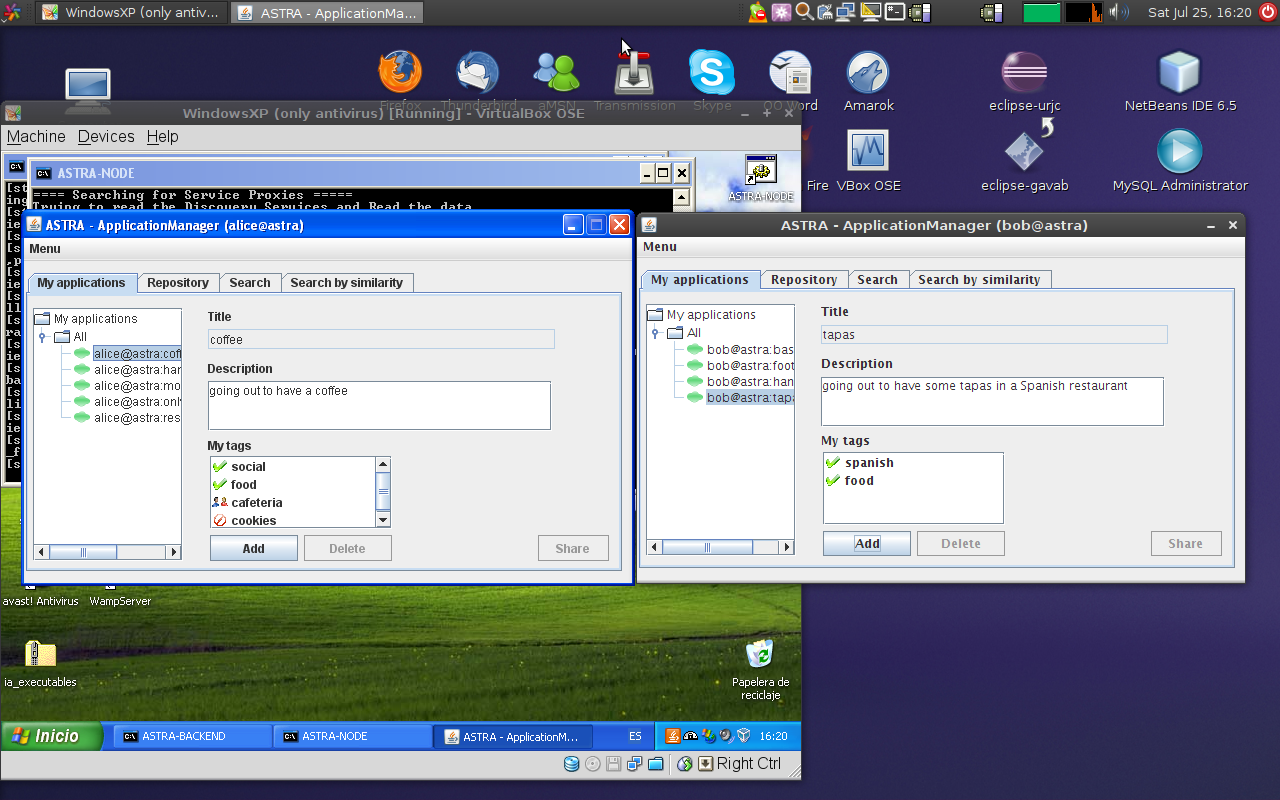
\includegraphics[scale=0.3]{screenshots/am-linux-w32.png}
 \end{center}
 \caption{\label{img:testing-win-linux}ApplicationManager running in GNU/Linux
 and Windows XP simultaneously}
\end{figure}

\subsection{Search engine testing}
\label{subsec:testing-search-engine}

In this section we will explain the process we carried on to evaluate the
search by similarity process. Since the origin of the data is totally
artificial (it was created by only one person) it does not intend to be a real
study, but it explains a possible way to evaluate it once data gathered from a
real set of users will be available.

We created a set of 25 applications, with a description and a set of 4 tags
for each of them. All these applications were under the ownership of an user
called \verb|"admin"| and shared in a community called \verb|"official"|. These
applications were divided into 5 groups: ``Sport'', ``Social'', ``Feelings'',
``Cultural'' and ``Location''. We assumed an application can only belong to one
of this groups to make the measuring process simpler, but this introduces an
error, since the way an application is categorized is subjective and not
exclusive. For example, an application \verb|admin@astra:concert| with
description ``going to a live music concert'' was classified into the group 
``Cultural", but for other people could be in the group ``Social" or even in
both. This will be taken into account when evaluating the results, since we will 
prefer to have a bigger recall even at the expense of loosing precision. The
raw data can be found in the Tables \ref{table:testing-data-sport}, 
\ref{table:testing-data-social}, \ref{table:testing-data-feelings}, 
\ref{table:testing-data-cultural} and \ref{table:testing-data-location} in
Appendix \ref{appendix:testing-search-engine-data}.

We created a new user afterwards that owns 5 applications which are similar (in
description and tags) to one of each of the groups. This will help us to
evaluate if we chose properly the fields to create the query and the fields to
perform the query in (see Section \ref{subsec:implementation-search-engine}).
As we explained in the previously referred section, the results are afterwards
sorted by score (see Appendix \ref{appendix:score-lucene} for more details in
scoring in Lucene).

The measures we took were:

\begin{itemize}
  \item \emph{RD}: Total number of retrieved documents.
  \item \emph{RDR}: Relevant documents retrieved.
  \item \emph{ERD}: Total number of existing relevant documents.
\end{itemize}

With these variables we can calculate the precision and recall percentage:
\[
precision = (RDR/RD)*100
\]

\[
recall = (RDR/ERD)*100
\]
%\\
%${\displaystyle recall = (RDR/ERD)*100}$\




Before taking the measures and perform the calculations, we defined a small set
of testing goals:
\begin{itemize}
  \item The application with the biggest score should be always the one it was
  based on. This acts as a ``control measure'' for the scoring.
  \item We should have a recall of at least 80\%.
  \item We should have a precision of at least 40\%.
\end{itemize}

The reason why we stressed on the recall values at the expense of the
precision is because of the nature of the categorization, as it was explained
before.

The measures and calculations for each application can be found in Tables
\ref{table:testing-results-sport}, \ref{table:testing-results-social},
\ref{table:testing-results-feelings}, \ref{table:testing-results-cultural} and
\ref{table:testing-results-location} in Appendix \ref{appendix:testing-search-engine-data}.

Table \ref{table:testing-summary} summarizes the calculations by groups and on
average.

\begin{table}[h!]
	\small
    \begin{center}
		\begin{tabular}{||c|c|c|c|c|c||}

		\hline \hline
			Group & RD & RDR & ERD & Precision & Recall \\
		\hline \hline
			Sport & 9 & 5 & 5 & 55.56\% & 100\%\\
			\hline
			Social & 10 & 5 & 5 & 50\% & 100\%\\
			\hline
			Feelings & 10 & 5 & 5 & 50\% & 100\%\\
			\hline
			Cultural & 7 & 4 & 5 & 57.14\% & 80\%\\
			\hline
			Location & 10 & 5 & 5 & 50\% & 100\%\\
			\hline
			\hline
			Average & 9.2 & 5 & 5 & 52.54\% & 96\%\\

		\hline \hline

		\end{tabular}
		\caption{\label{table:testing-summary} Summary of the results for search by
		similarity evaluation}
	\end{center}
\end{table}

From this simple evaluation, we can remark:

\begin{itemize}
  \item It satisfies the preliminary testing goals, with a 96\% average in
  recall and 52.54\% average in precision. It also satisfies the ``control
  group'' goal in all the cases.
  \item In most of the cases, the 5 first results belong to the group we were
  expecting (see Appendix \ref{appendix:testing-search-engine-data}). This could
  be useful to establish a threshold in case the precision will decrease too
  much in the future.
  \item When there are false positives, in general all of them belong to
  no more than one or two of the categories (see for instance
  Table \ref{table:testing-results-feelings}). This can be explained because of
  the rigid way we have tagged and categorized the applications in
  contrast with the intrinsic non-exclusive nature of the applications
  categorization.
\end{itemize}

It is important to remark that the data was totally artificial, therefore the
aim of this small evaluation was just assuring the design decisions point to the
right way, and to establish a possible way of measuring in the future.


\subsection{Users evaluation}
\label{subsubsec:testing-users-study}

A preliminary users evaluation after iterations 1 and 2 (see Table
\ref{table:iterations}) was performed at NTNU in Trondheim (Norway) on the 13th
of December 2008. There were 8 participants, all of them exchange students
since those represent one of the main scenarios in ASTRA.
A deep analysis is beyond the scope of this document (detailed information can
be found in \cite{astra-repo}), but we will summarize the most important ideas
and impressions given by the users, and the way we have used this feedback for
developing the current version of the project:

\begin{itemize}
  \item Participants were positive about the idea of sharing and 
 		getting applications.
  \item The notion of community had a good reception, and they evaluated
  positively the visibility in terms of community. This feedback has been taken
  into account in iterations 3 and 4 (i.e.: adding support to browse by
  communities in local and remote applications).
  \item The search functionalities needed to be extended. This is one of the
  main features added in iteration 3 with the integration of a search engine
  into the repository.
  \item Users evaluate very positively the possibility of having public and
  community tags. Users also pointed the necessity of removing them, which is
  supported in the current version.
  \item Users evaluate positively the introduction of ontologies. For instance
  this can be used to support a better categorization. This issue is part
  of the future work (see Section \ref{sec:future-work}), and the bundles
  developed for this project are already integrated with
  \verb|OntologyManager|'s interface, so they will work once that
  functionalities are implemented in that bundle.
  \item Some privacy issues arise, regarding especially the need of removing
  rules. For instance, an application may have a rule which provides
  information about our location that we do not want to share.
  This has been addressed in the current version, in which we provide mechanisms
  to visualize and adapt the application (i.e.: discard a rule after 
  visualizing its auto-generated description), so the users can handle its
  privacy.
  \item Implementing a search by similarity from a recommended application was
  pointed as an interesting option. This is addressed in the current version.
\end{itemize}

A new users evaluation at NTNU including the work performed during iterations 3
and 4 is scheduled in October 2009, once some other ASTRA components will be
developed, so they can also be tested in the same evaluation.
